%! Author = paulsen
%! Date = 12.09.23

\begin{frame}
    \frametitle{Test}


    \section{Testsection}\label{sec:testsection}

    \begin{quote}
        Lorem ipsum dolor sit amet, consectetur adipisicing elit
    \end{quote}

    \begin{tikzpicture}
        [remember picture,overlay,shift={(current page.north east)}]
        \node[anchor=north east,xshift=-7cm,yshift=-2.5cm]{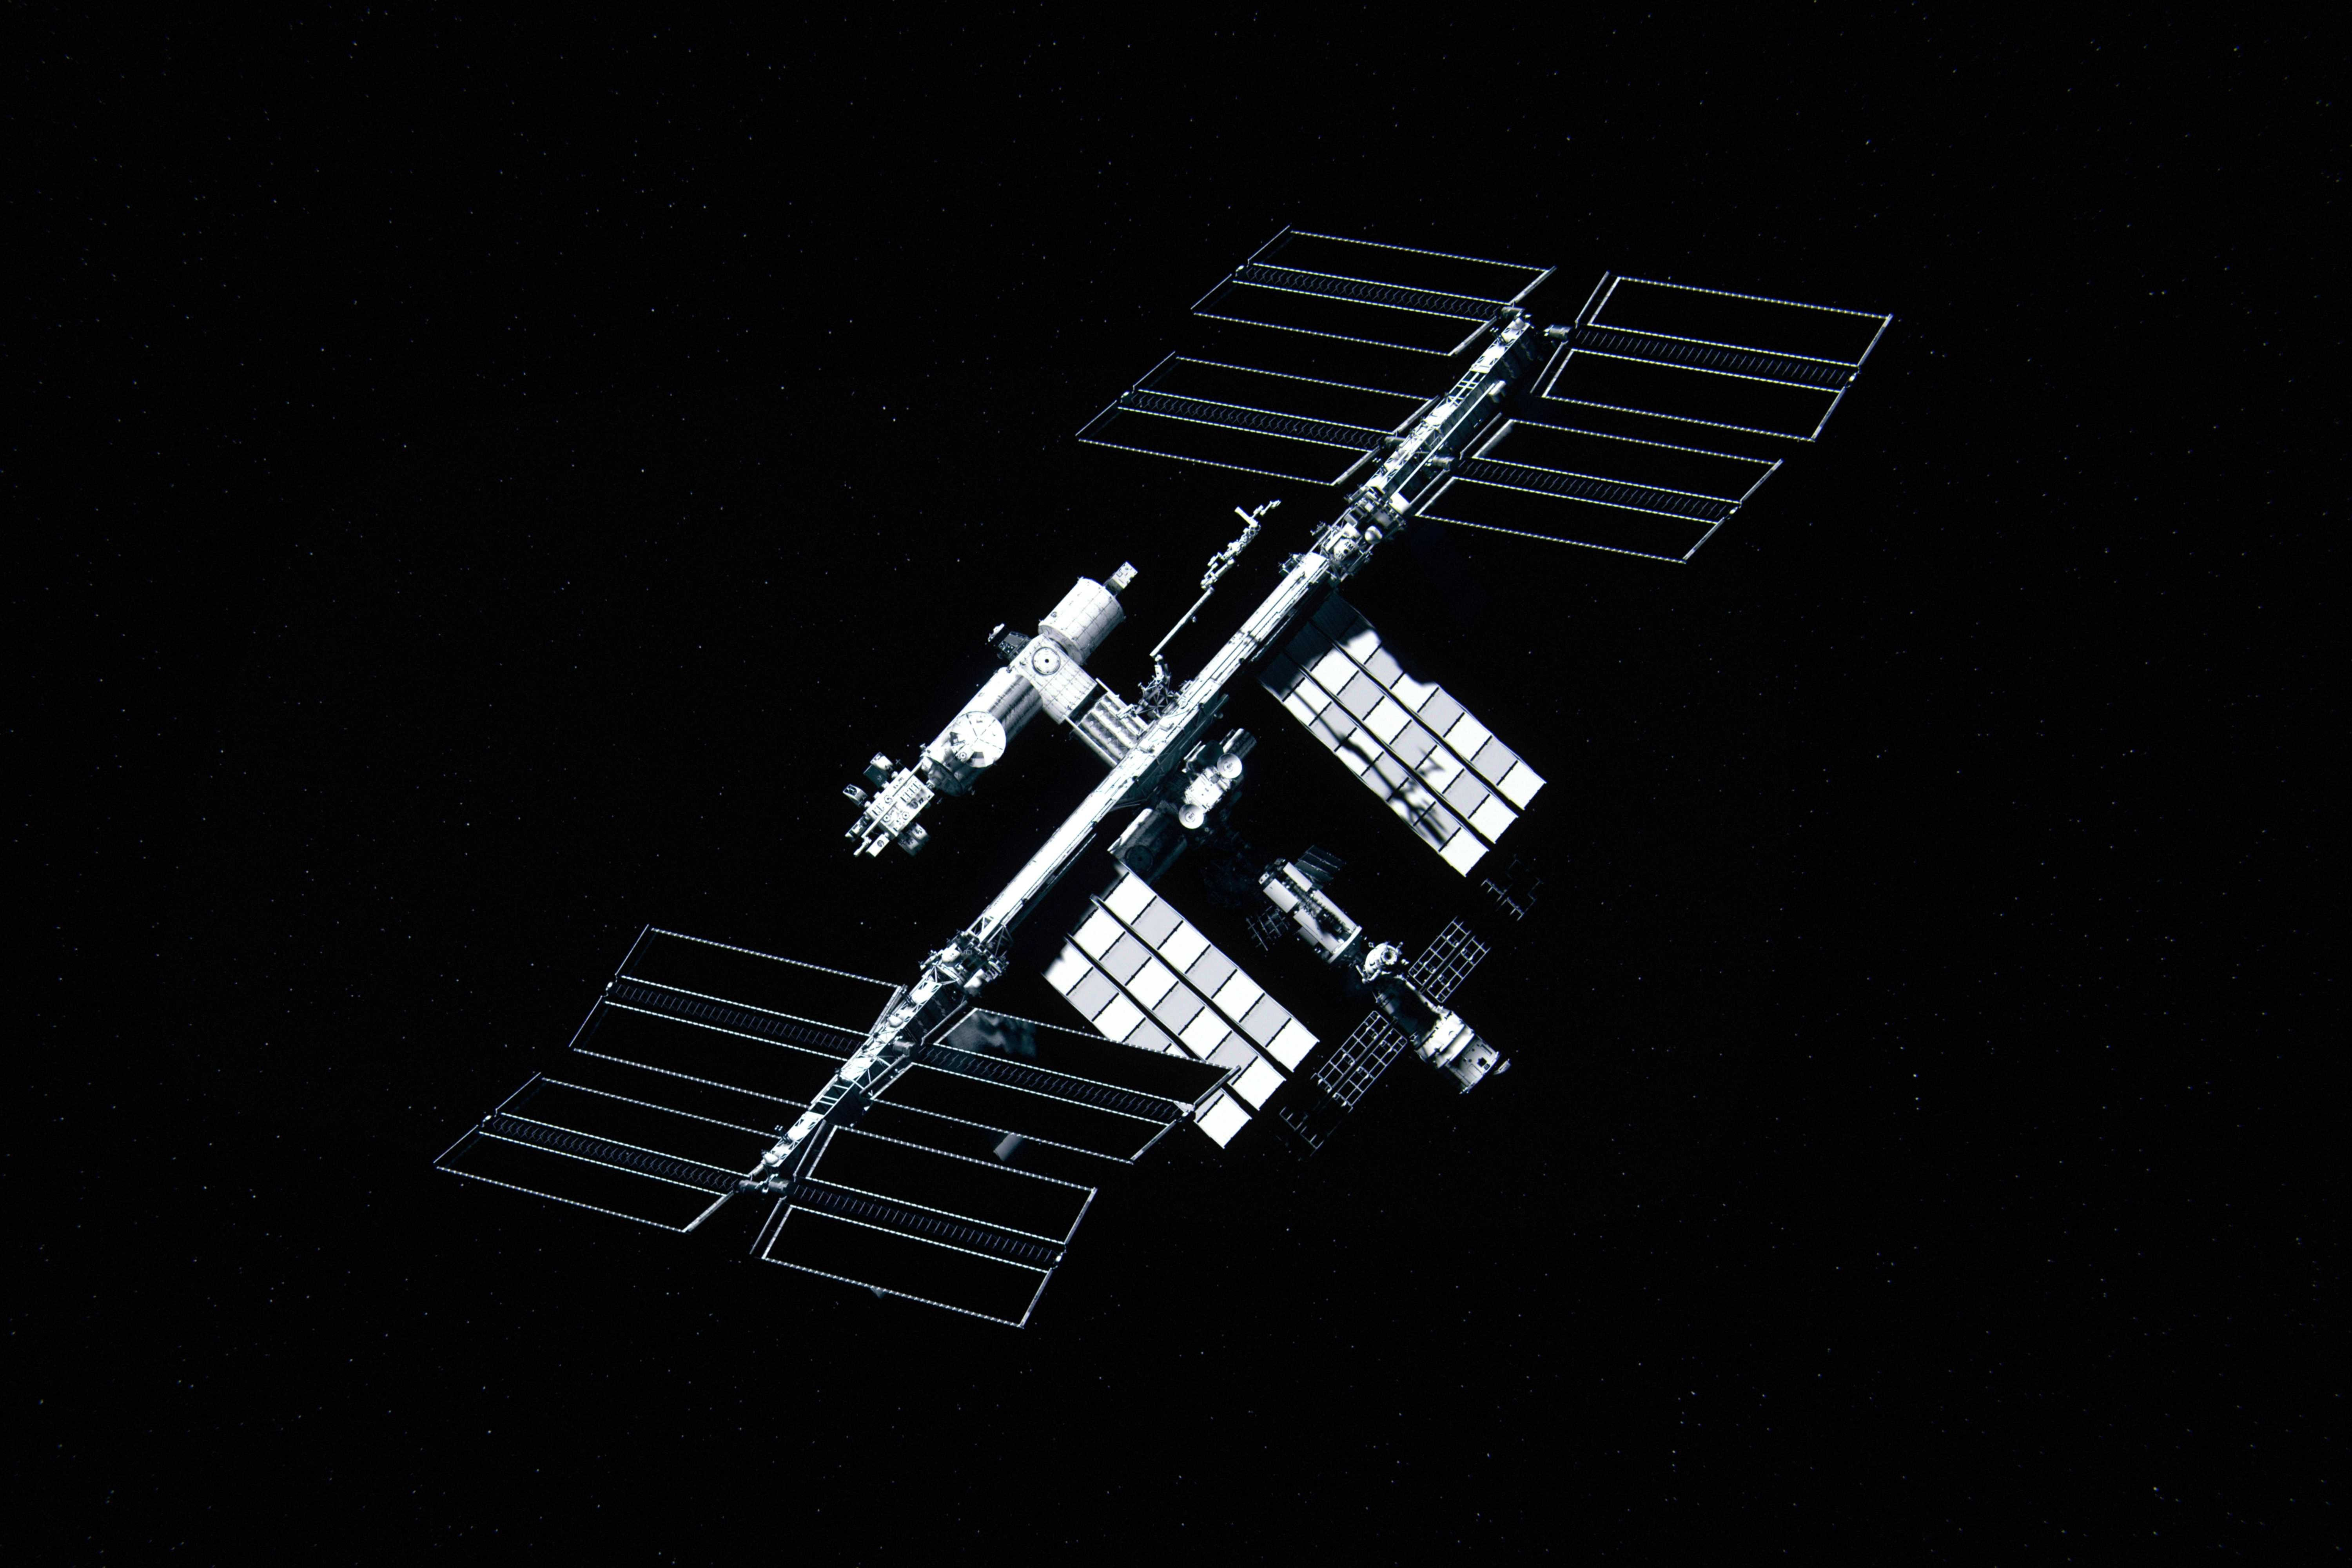
\includegraphics[width=2cm]{ISS}};
        \node[anchor=north east,xshift=-5cm,yshift=-2.5cm]{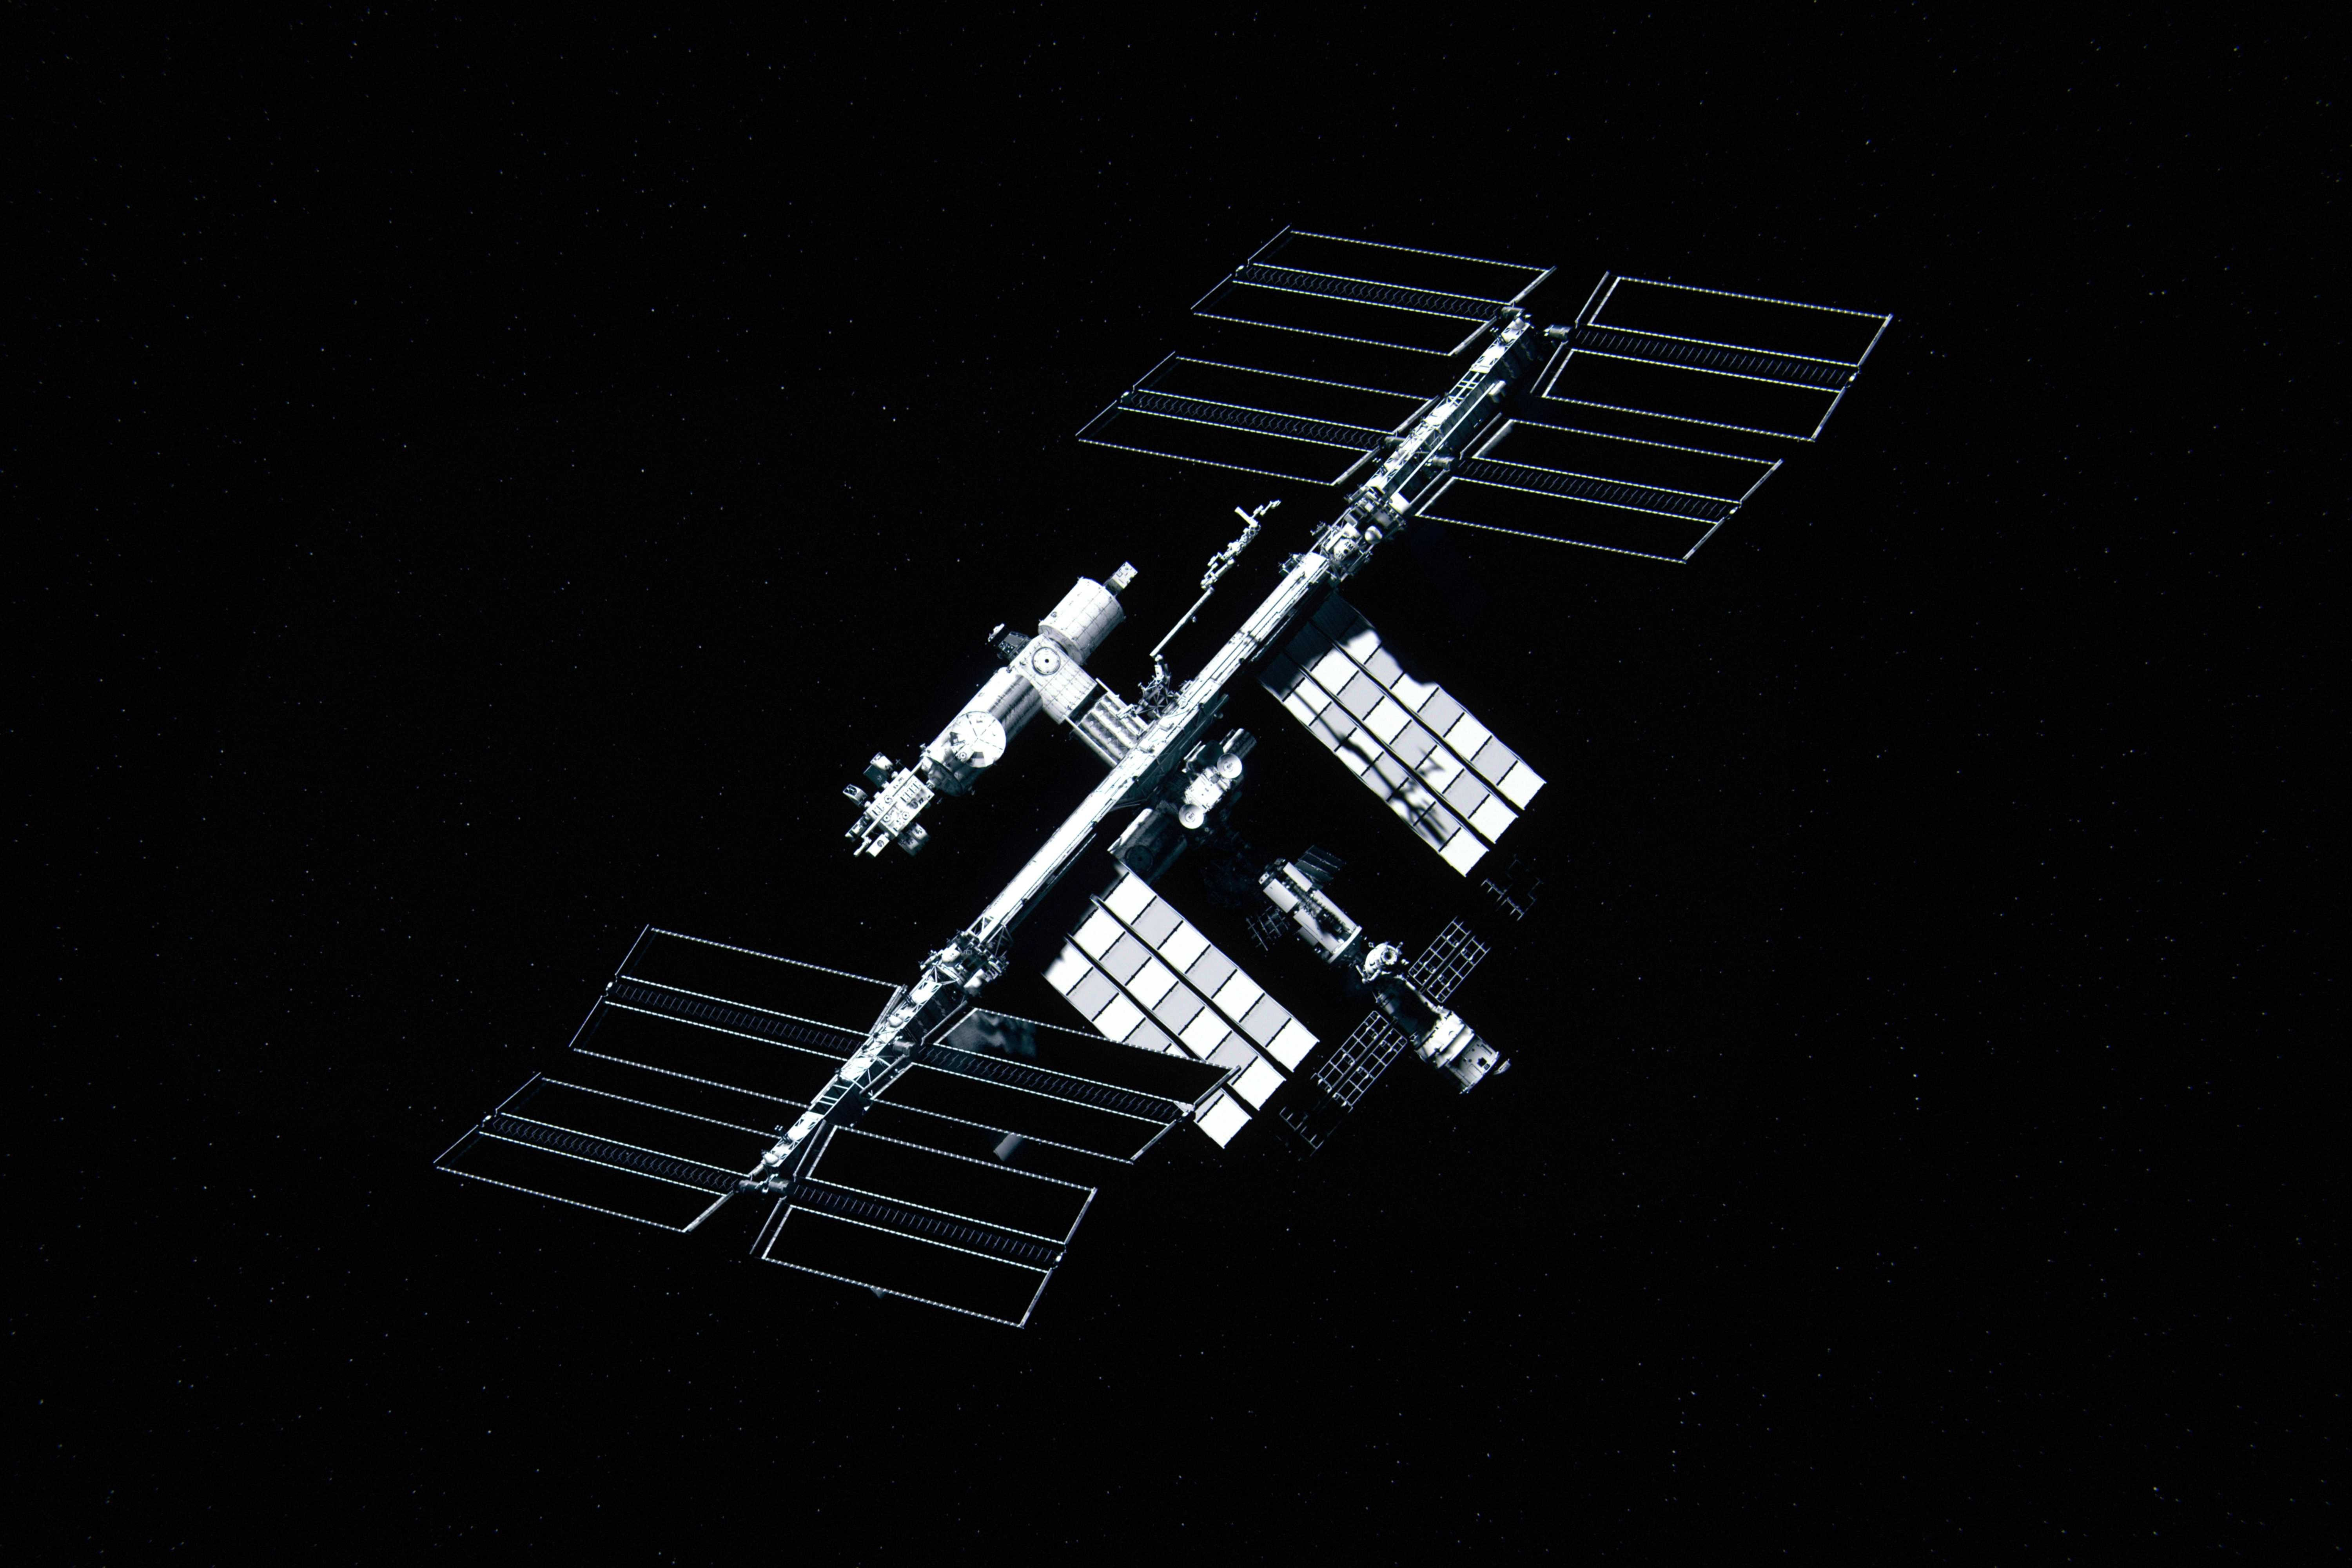
\includegraphics[width=3cm]{ISS}};
        \node[anchor=north east,xshift=-1cm,yshift=-2.5cm]{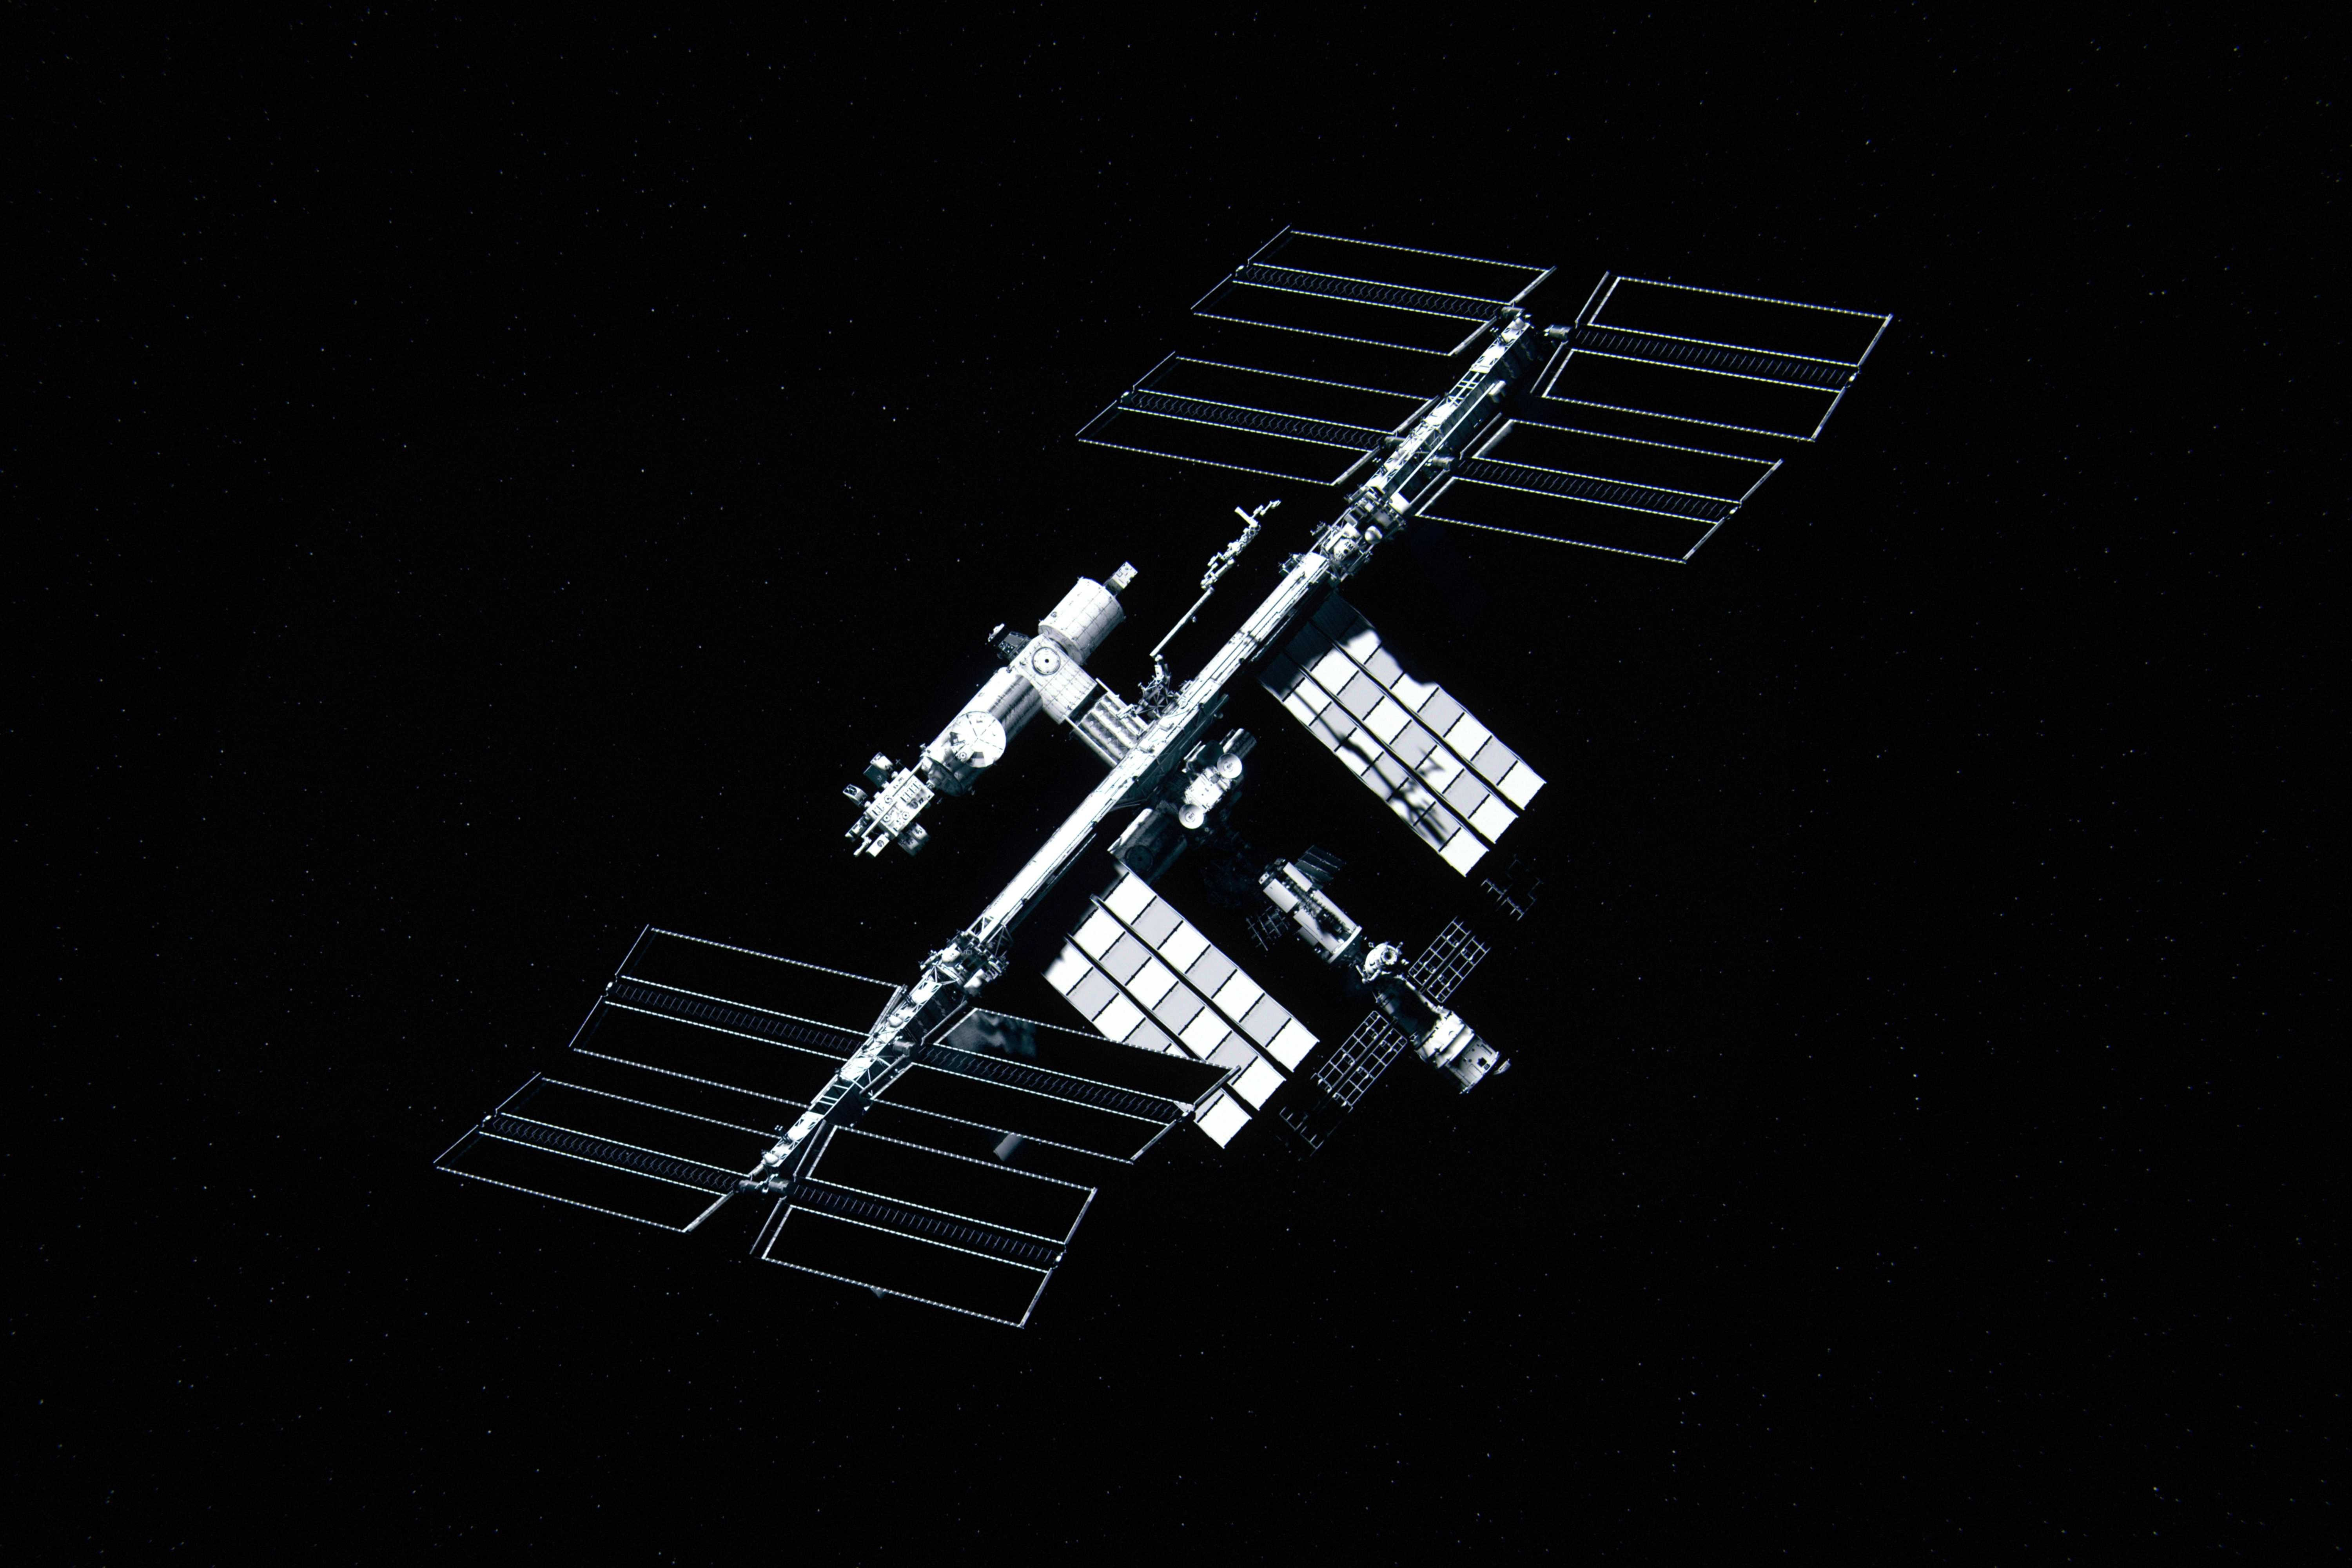
\includegraphics[width=5cm]{ISS}};
    \end{tikzpicture}

    \subsection{Listen}\label{subsec:Listen}
    \begin{itemize}
        \item[!.] Eintrag
        \begin{enumerate}
            \item Test123
        \end{enumerate}
        \item Descriptions
        \begin{description}
            \item<2->[Thema] Schilderung
        \end{description}
    \end{itemize}

    \subsection{Blöcke}\label{subsec:Blocke}
    \begin{alertblock}{Beispiel 1}
        Die ISS ist schön
    \end{alertblock}
    \begin{exampleblock}{Fun Fact}
        Die ISS läuft mit Linux.
    \end{exampleblock}

\end{frame}